\chapter{Results and Tests}
\label{chap:results}
\section{Program}
The final version of the program features a simple button-to-LED mapping. The gamepad (seen on figure \ref{img:gamepad}), has 8 buttons and 8 LEDs, both sets indexed 1 through 8. Pushing button $N$ activates LED $N$. The nature of the program allows any number of buttons to be simultaneously pressed and the corresponding LEDs to be activated.

\subsection{Testing the program}
All tests require possession of an EFM32GG-DK3750, a purpose built gamepad connected to the board on GPIO ports A and C and a computer capable of compiling for arm based platforms and flashing software to the development board.

\subsubsection{Button functionality test}

This procedure tests the implemented functionality of our program. Pushing button $N$ should light LED $N$.

Procedure:

\begin{enumerate}
\item Compile and flash the program to the board by running \texttt{make run} from the project root
\item Wait for the board to reset properly
\item Push each button, ensuring the corresponding LED lights up.
\end{enumerate}


\section{Energy efficiency}
When we discuss energy efficiency, we will primarily be looking at the current spent (amperage). Wattage or voltage could have been investigated too, but amperage is the most interesting because it can be more easily related to things such as battery capacity. The current powering the LEDs is not registered, as the jumper on the gamepad is set to "disabled" (see section \ref{devices}).

\subsection{Readings}
Using the eAProfiler monitoring tool we observed the graph oscillating around and averaging about $2.0 \mu A$ while running the final iteration of the program with sleep mode enabled. Previously we had seen it average slightly lower, about $1.6 \mu A$. We assume that this is because the temperature of the room increased, thus increasing the temperature of the components in the system and causing conductivity to decrease. Unfortunately we did not have the time to run the sleeping program for an extended time in a regulated temperature, so we had to make do with the $2.0 \mu A$ reading as our main data point.

Figure \ref{fig:ampsplot} shows the plot of the amperage on a log scale. First no buttons are pressed, then one, two, three and four. The amperage while these we pushed are shown in table \ref{tbl:current}.

\begin{figure}[h!]
    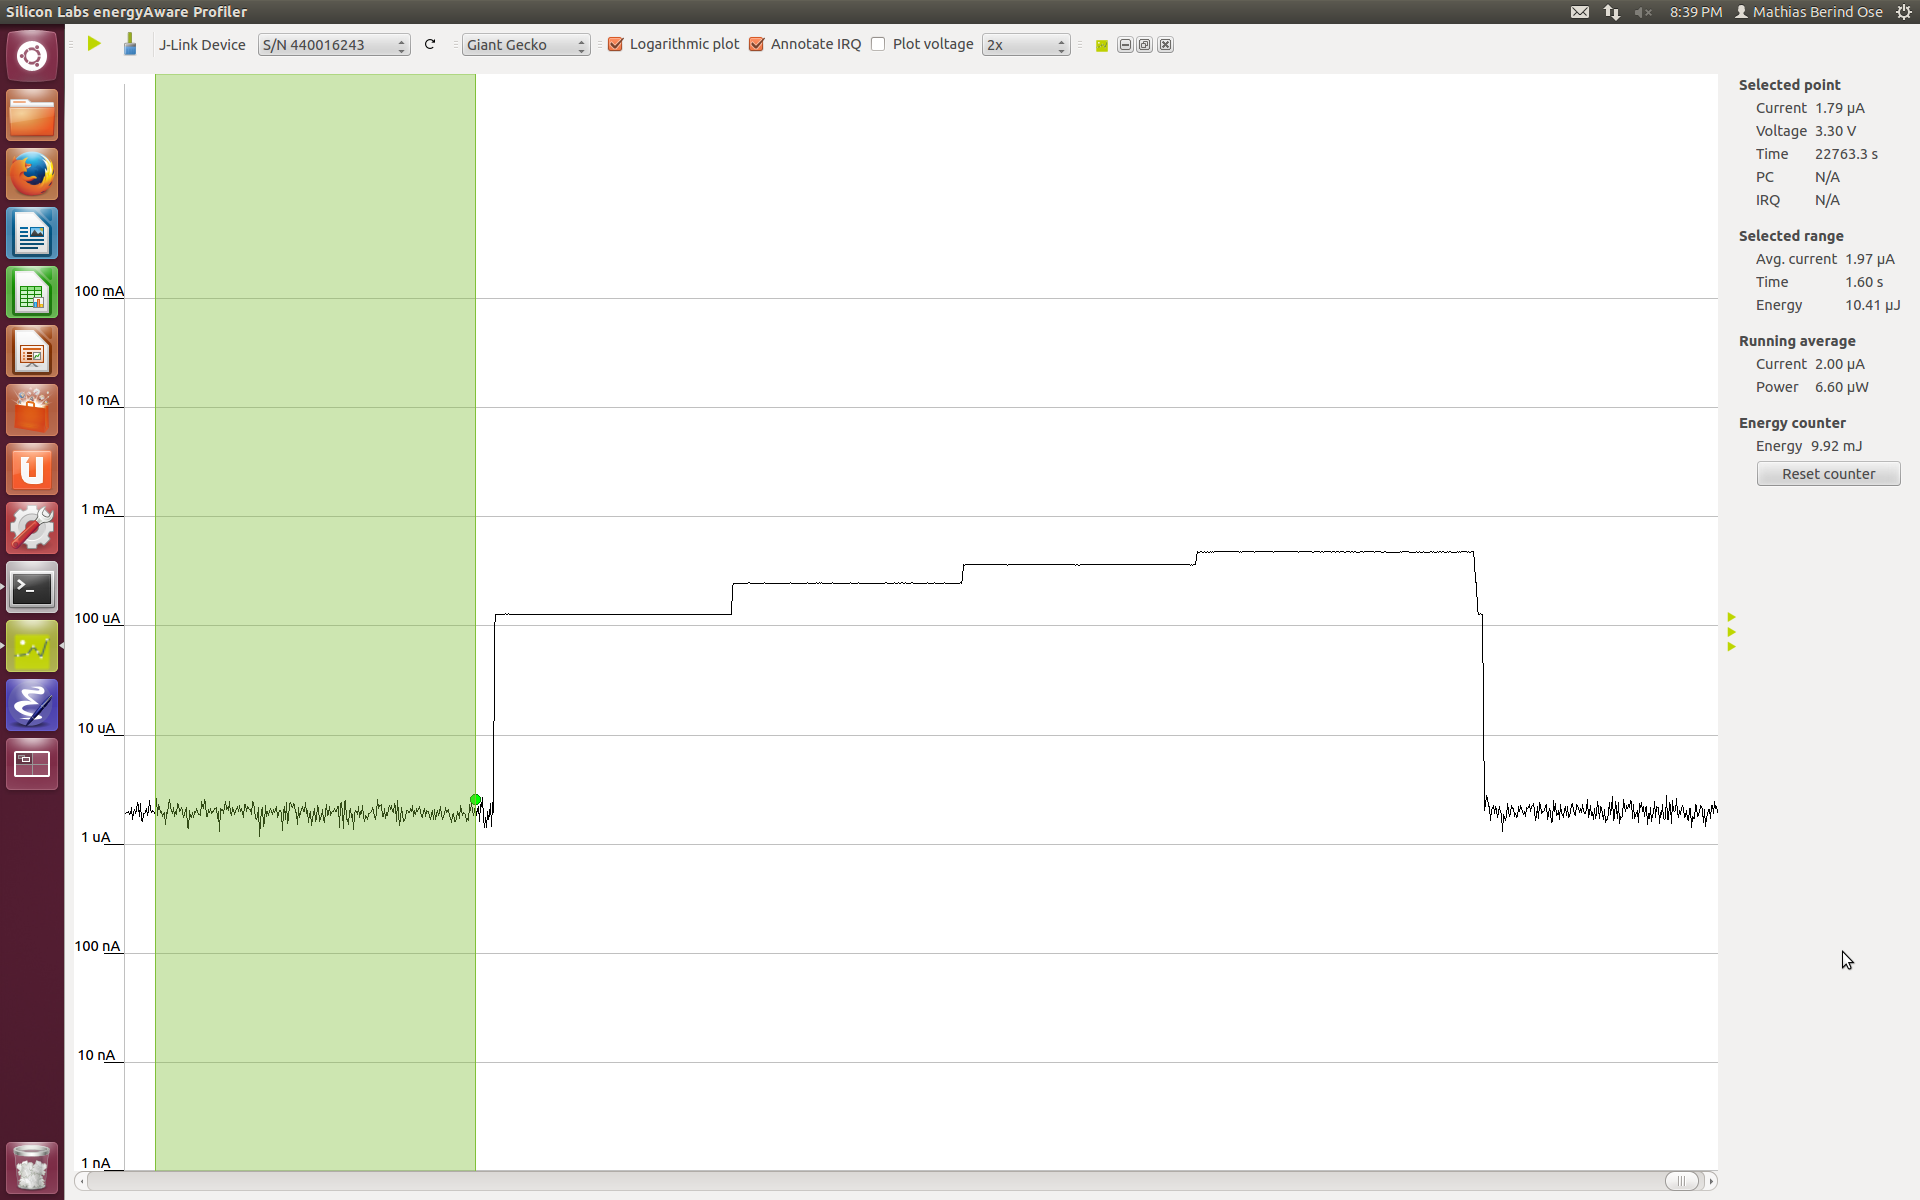
\includegraphics[width=\linewidth]{img/0.png}
    \caption{The amperage plotted by the eAProfiler tool.}
    \label{fig:ampsplot}
\end{figure}
\begin{table}[h!]
    \begin{tabular}{l|l}
        Buttons pressed & Current [$\mu A$] \\
	\hline
	0               & 1.97              \\
	1               & 130.41            \\
        2               & 260.85            \\
	3               & 364.33            \\
	4               & 476.34
    \end{tabular}
    \caption{Buttons pressed and resulting amperage \label{tbl:current}}
\end{table}

When running the build with polling instead of interrupts, the amperage averaged $3.6 mA$. That means that the idling system uses 1800 times more current than the sleeping version.

\subsection{Expected lifetime on a cr2032 battery}

Representatives from Silicon Labs, the manufacturer of the EFM32GG STK have used the cr2032 "coin cell" battery as an example when talking about the energy efficiency of their products. For this reason we chose to look up some statistics about this battery online and calculate the theoretical time the development board can run on one battery. One battery manufacturer claims their battery has a typical capacity of $240 mAh$.\cite{cr2032spec}

\[
	240 mAh / 2.0 uA = 120 000 \text{~hours} = 5000 \text{~days} = 13.7 \text{~years}
\]

According to one source \cite{cr2032} a coin cell battery can last up to 5 years while in use before deteriorating too much. In other words the battery will deteriorate before discharging from use for this microcontroller running this sleeping program.

If the polling version of the program had been running instead, the coin cell battery would only last 2 days and 18 hours.

\section{Discussion}
The primary goal of the exercise was learning, and that was definently achieved. The group members had no significant prior experience with the technologies, only some theoretical knowledge from the TDT4160 course. But thanks to the instructions in the compendium we were able to do most of the work on our own.

The biggest problem we had was enabling sleep mode with interrupt-based I/O. After following the instructions in the compendium we had sucessfully implemented the I/O with interrupts, but the microcontroller did not go to sleep mode. Attempts at debugging revealed that removing code crucial to the I/O made the device go to sleep. It seemed impossible to solve the problem, but inexplicably it suddenly began working after moving some code about, even though it seems that should not have changed anything (See section \ref{sec:energy-optimization}). We spent hours debugging the issue, but at the time of writing we have yet to reach a conclusion as to why it worked out the way it did. One theory arose after placing the deep sleep configuration code back into the reset subroutine, and placing three \texttt{NOP} instructions above it. Doing this made everything work smoothly, leading us to thinking that perhaps the instruction pipeline has to be cleared before one can write to the SCR register. This could however not be confirmed by subject staff or inquiries into the documentation of the processor.
